% ------------------------------------------------------------------------
% -*-TeX-*- -*-Hard-*- Smart Wrapping
% ------------------------------------------------------------------------
\def\baselinestretch{1}

\chapter{Literature Review}

\def\baselinestretch{1.44}

%%% ----------------------------------------------------------------------

   
\smallskip

%%% ----------------------------------------------------------------------
\goodbreak
\section{Overview Of Bitcoin Trading}
\smallskip

%%% ----------------------------------------------------------------------
\goodbreak

\subsection{Historical Perspective}
A person or group of persons using the alias Satoshi Nakamoto conceptualized Bitcoin, commonly referred to as a cryptocurrency, in a white paper in 2008. Later, in 2009, it was made available as open-source software \citep{article}. Bitcoin uses a decentralized network of computers, as opposed to conventional currencies that are issued by governments and central banks, and it uses blockchain technology to record and validate transactions.

As a technological novelty rather than a commonly used medium of trade in its early years, Bitcoin. In 2010, a programmer bought two pizzas for 10,000 Bitcoins in the first recorded commercial use of Bitcoin (Hern, 2013). The Bitcoin community famously observes this day as "Bitcoin Pizza Day."


The popularity and value of Bitcoin, however, started to soar after 2011, especially after it gained acceptance on platforms like WordPress, Microsoft, and major e-commerce websites. When Bitcoin reached an all-time high of around 20,000 dollars in 2017, it was a huge turning point. However, the following years saw extraordinary volatility (Chapman et al., 2018).

\begin{figure}[H]
\centering
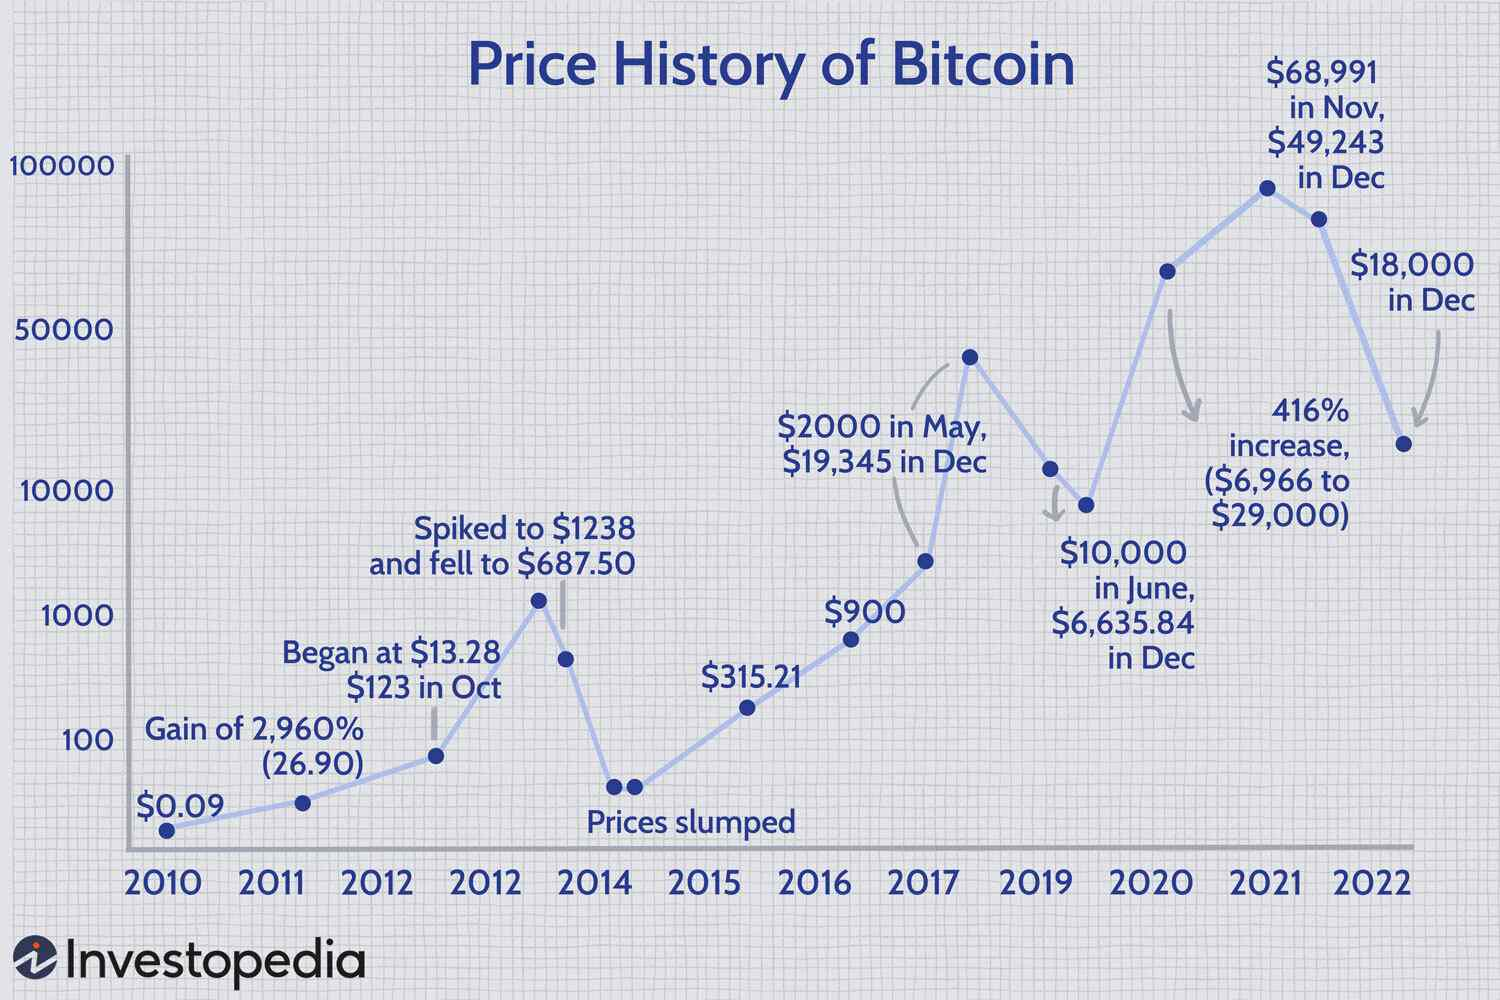
\includegraphics[scale=0.25]{Fig1.jpg}
\caption{Bitcoin Price Trend Overtime.}
\citep{noauthor_bitcoins_nodate}
\end{figure}



\subsection{Market Dynamics and Behavior}
Numerous internal and extrinsic factors, as well as market conditions, have an impact on Bitcoin's price dynamics. Unlike conventional financial assets, Bitcoin's valuation is not determined by cash flows, dividends, or interest payments. Alternatively, it is frequently compared to commodities like gold, acting as a store of value or "digital gold" \citep{DBLP:conf/ecis/GlaserZHW14}.
\smallskip

%%% ----------------------------------------------------------------------
Several factors impact Bitcoin's price:
\smallskip

%%% ----------------------------------------------------------------------
\textbf{Supply and Demand:} The total number of Bitcoin coins in circulation is 21 million. Given the shortage and rising demand, particularly from institutional investors, which can then lead to an overall price surge. \citep{DBLP:journals/ijecommerce/PolasikPWKL15}

\smallskip

\textbf{Regulatory News:} The price of Bitcoin can be significantly impacted by governmental rules or simply by the prospect of upcoming regulations. For instance, price reductions have typically been precipitated by regulatory crackdowns in nations like China \citep{feng_informed_2018}.

\smallskip

\textbf{Technological Changes and Innovations:} Technological developments in the blockchain industry or scaling solutions like the Lightning Network might affect investor sentiment and the price of Bitcoin. \citep{easley_mining_2019}

\smallskip

\textbf{Macroeconomic factors:} It can affect the price of decentralized assets like Bitcoin by increasing their allure. These factors include economic downturns, inflation rates, and political unrest. \citep{urquhart_inefficiency_2016}.

\smallskip

Markets for bitcoin are notorious for their high volatility. Its speculative nature, restricted liquidity, regulatory news, and macroeconomic factors might be blamed for this volatility. Furthermore, the actions of Bitcoin traders, particularly those motivated by herd behavior, worsen this volatility. \citep{bouri_hedge_2017}.

\goodbreak

\section{Machine Learning in Financial Computing}
\goodbreak

\subsection{Applications and Techniques:}

Over the past ten years, \gls{ml} has significantly advanced in the field of financial computing. Its uses are many, using sophisticated algorithms to inform choices, forecast market movements, spot fraud, and more.

\smallskip

\textbf{Portfolio Management (Robo-Advisors):}

The asset portfolios of customers are automatically allocated, managed, and optimized by robo-advisors using ML approaches in accordance with their unique preferences and goals. \gls{ml} models can optimize asset allocation more effectively than conventional techniques by analyzing enormous volumes of data \citep{goldstein_investor_2017}.

\smallskip

\textbf{Algorithmic Trading:}

High-frequency trading companies use ML algorithms to forecast price fluctuations on a millisecond time scale. These forecasts are based on massive databases, which also include order books, trading volumes, and even news items. Deep learning and neural networks have both proven extremely useful in this domain. \citep{DBLP:journals/cacm/TreleavenGL13}

\smallskip

\textbf{Credit Scoring:} 

Conventional credit scoring techniques frequently use manual procedures and standards based on rules. These models can be improved by \gls{ml}, which analyses a wider variety of data (including non-traditional data) and more accurately predicts the likelihood of defaults \citep{DBLP:journals/eor/LessmannBST15}.

\smallskip

\textbf{Fraud Detection:} 

\gls{ml} models can be taught to find patterns linked to fraudulent transactions. These algorithms can adapt and identify novel, previously unidentified types of fraud by continuously learning from fresh transactions \citep{10.1214/ss/1042727940}.

\goodbreak



\textbf{Risk management:} 

\gls{ml} can help, especially with complex financial products, in comprehending and managing risk. \gls{ml} models can offer more precise risk evaluations and even forecast probable market downturns by examining market conditions and historical data \citep{DBLP:journals/eswa/YehYT09}.

\begin{table}[H]
\centering
\begin{tabular}{|l|l|p{5cm}|}
\hline
\textbf{Applications} & \textbf{Tree-based Ensembles} & \textbf{Deep Learning Models} \\
\hline
Credit Scoring & Widely used & Emerging use \\
\hline
Fraud Detection & Commonly used & Widely used with neural networks \\
\hline
Algorithmic Trading & Used & More common with time-series data \\
\hline
Portfolio Management & Used & Emerging use
with reinforcement Learning \\
\hline
Risk Management & Widely used & Emerging use \\
\hline
\end{tabular}
\caption{Applications of Tree-based Ensembles and Deep Learning Models in Finance}
\citep{ravi2015survey}
\label{table:applications_comparison}
\end{table}

\goodbreak

\subsection{Opportunities and Challenges:}

\smallskip

Although ML has tremendous prospects for financial computing, it also poses difficulties:

\textbf{Data Quantity and Availability:}
 The effectiveness of ML models is strongly influenced by the quality and quantity of accessible data. When training robust models, financial institutions may struggle with inconsistent, missing, or unstructured data \citep{DBLP:journals/mansci/BaesensSMV03}.

\smallskip
 
\textbf{Interpretability: }
A lot of sophisticated ML models, particularly deep learning models, lack interpretability. The "black-box" character of some ML models raises questions in a field where decisions might have large financial repercussions \citep{DBLP:conf/kdd/Ribeiro0G16}.

\smallskip

\textbf{Overfitting:} 
There is a chance that ML models will become overly reliant on previous data, which will limit their ability to adapt to novel, unforeseen market conditions. Decisions made as a result of overfitting may not be the best ones \citep{DBLP:journals/jcisd/HawkinsBM03}.

\smallskip

However, these difficulties also present chances:

\smallskip

\textbf{Data engineering Solutions:} It can be used to ensure consistent, high-quality data for training, hence addressing the problem of poor data quality (Wang  Strong, 1996).

\smallskip

\textbf{Explainable \gls{ai}:} There is rising interest in creating sophisticated models that can also be understood. To increase the transparency of ML models, explainable \gls{ai}  techniques have been developed \citep{doshivelez2017rigorous}.

\smallskip

\textbf{Regularization Techniques:} It can be used to prevent overfitting and make sure that models generalize properly to fresh data \citep{10.1145/1015330.1015435}.

\goodbreak
\section{Tree-based Ensembles in Predictive Modeling}
\smallskip

%%% ----------------------------------------------------------------------
\goodbreak

\subsection{Random Forest in Finance}


In finance, the ensemble learning technique Random Forest can be applied to both classification and regression applications. To create more reliable forecasts, it mixes different decision trees \citep{breiman_random_2001}.

\textbf{Stock Price Prediction:} Random Forest has been used to forecast stock price changes, and many tests have found it to be highly accurate \citep{liaw2002classification}.

\textbf{Credit Risk Assessment:} The model has also been employed to assess borrowers' creditworthiness \citep{DBLP:conf/kdd/ChenG16}.

\goodbreak

\subsection{Other Ensemble Methods:}

Other popular tree-based ensemble techniques in the finance industry include:

\textbf{Gradient Boosting:} According to \cite{4a848dd1-54e3-3c3c-83c3-04977ded2e71}, this technique creates trees one at a time, fixing the mistakes of the preceding ones.

\textbf{AdaBoost:} It is a different boosting technique that is focused on difficult-to-predict situations \citep{DBLP:conf/icml/FreundS96}.

\textbf{XGBoost:} It is a gradient boosting extension that is renowned for its computational effectiveness \citep{DBLP:conf/kdd/ChenG16}.



\subsection{Performance Metrics:} 

\goodbreak

 The validation of a model's effectiveness is, as much as it is the modeling itself, an important factor for prediction models that are especially applicable to finance applications. A set of performance metrics shall be used to determine the reliability and precision of the model. These measures provide a quantitative assessment of the model's assumptions, as opposed to its actual results.


\textbf{Accuracy:}   Accuracy calculates the proportion of accurately predicted instances to all instances, making it the most simple metric. Accuracy can be deceptive, even though it offers a preliminary assessment of model performance, particularly in unbalanced datasets where one class is disproportionately overrepresented  \citep{M2015ARO}.

\[ \text{Accuracy} = \frac{\text{Number of correct predictions}}{\text{Total number of predictions}} \]

\textbf{Precision and Recall:} It rates the precision of correct predictions. An algorithm with great precision will have returned significantly more relevant results than irrelevant ones. and Recall calculates what percentage of all relevant instances were actually retrieved. When the cost of missing a favorable instance is high, it is essential.
 \citep{DBLP:journals/corr/abs-2010-16061}.

\[ \text{Precision} = \frac{\text{True Positives}}{\text{True Positives} + \text{False Positives}} \]

\[ \text{Recall} = \frac{\text{True Positives}}{\text{True Positives} + \text{False Negatives}} \]

\textbf{F1 Score:} The F1 Score is a harmonic average of precision and recall that mediates the balance between precision and recall. F1 scores closer to one mean better precision and performance balance\citep{DBLP:journals/ipm/SokolovaL09}.

\[ F1 = 2 \times \frac{\text{Precision} \times \text{Recall}}{\text{Precision} + \text{Recall}} \]


\textbf{Root Mean Square Error(RMSE):}

For regression problems or financial forecasting, \gls{rmse} measures how accurately the model predicts the outcome. This gives an idea of the size of the error between the predicted and observed values.

\[ \text{RMSE} = \sqrt{\frac{1}{n} \sum_{i=1}^{n} (y_i - \hat{y}_i)^2} \]

\textbf{\gls{auc}:}
 In the case of classification problems, the \gls{auc} of the receiver operating characteristic \gls{roc} curve is an essential metric. The ability of the model to distinguish between positive and negative classes is illustrated. A more refined model is implied by an \gls{auc} closer to 1.

\goodbreak
\section{Deep Learning Models for Trading Analysis}
\smallskip

%%% ----------------------------------------------------------------------
\subsection{LSTM and Time Series Prediction}
\goodbreak

Recurrent Neural Networks (RNN) Long Short-Term Memory (LSTM) networks are crucial for forecasting time-series data. They have a wide range of uses in the financial markets, particularly for predicting price movements in the trading of bitcoins:

\textbf{Application In Bitcoin Trading:} According to \cite{DBLP:conf/nips/SutskeverVL14}, LSTM models are used to identify long-term dependencies and sequential information in Bitcoin price data. This helps to make precise predictions.


\textbf{Strengths and Limitations:} While LSTMs provide a sophisticated understanding of time-dependent data structures, their usefulness may be limited by the processing requirements and difficult hyperparameter tuning \citep{DBLP:journals/corr/ChungGCB14}.


\textbf{Comparison with Other Models:} According to \cite{DBLP:journals/neco/GersSC00}, LSTM frequently offers greater forecasting performance in erratic markets like Bitcoin. This is demonstrated by a comparison between LSTM and conventional time-series models like ARIMA.

\subsection{Modern Tools and Innovations} 

\goodbreak

With new developments, the use of deep learning in Bitcoin trading analysis continues to advance:

\textbf{\gls{drl}: }According to \cite{DBLP:journals/nature/MnihKSRVBGRFOPB15}, DRL has become a potent tool for optimizing trading tactics in Bitcoin markets by dynamically adjusting to market changes.

\textbf{Pre-trained Models:} Using pre-trained models for sentiment research, such as BERT, has revealed fresh information about market patterns in the bitcoin industry \citep{DBLP:journals/corr/abs-1810-04805}.

\textbf{Tools and Frameworks:} In the context of Bitcoin trading, frameworks like TensorFlow and PyTorch have made deep learning model deployment and experimentation more accessible \citep{DBLP:journals/corr/AbadiABBCCCDDDG16}\citep{DBLP:journals/corr/abs-1912-01703}.

\goodbreak
\section{Economic and Statistical Metrics for Evaluation}
\smallskip

%%% ----------------------------------------------------------------------
\subsection{Traditional Statistical Metrics}
\smallskip

Common metrics for measuring prediction mistakes, particularly in continuous forecasts like price trends, include mean squared error (MSE) and root mean square error (RMSE) \citep{hyndman_another_2006}.

\textbf{Accuracy, Precision, Recall, and F1-Score:} When the prediction job is stated as categorization, such as predicting upward or downward market movements, accuracy, precision, recall, and F1-Score metrics can be used \citep{DBLP:journals/ipm/SokolovaL09}.

\textbf{Time Series Specific Metrics:} Metrics Particular to Time Series: According to\citep{9f5faea9a4884eff9665c32105db424f}, time series forecasting is particularly relevant to specialised metrics like Mean Absolute Percentage Error (MAPE).

\subsection{Economical Significance}
\smallskip

\textbf{Profit and Loss Evaluation:} Metrics that measure the financial gains from implementing the model's predictions in actual trading scenarios.

\textbf{Metrics Based on Utility:} 
Taking into account the risk against benefit trade-off in relation to financial trading and investing \citep{danielsson_model_2016}.

\textbf{Market Impact Assessment:} Analysing the models in light of possible market effects including those on volatility and liquidity.

\subsection{Comparison Across Models}
\smallskip

\textbf{Statistical Tests for Comparing Models:} Methods for statistically comparing the performance of several models to identify significant differences, such as the Diebold-Mariano test \citep{doi:10.1080/07350015.1995.10524599}.

\textbf{Economic Value of Predictive Accuracy:} Models are evaluated not only for their statistical significance but also for their usefulness to traders and investors \citep{26d24c7c-b91e-306e-b000-d5246fb6c3cb}.

\goodbreak
\section{Summary of the Literature Gap}
\goodbreak

\subsection{Lack of Comprehensive Comparative Studies}
\goodbreak

There may be a dearth of thorough studies that systematically evaluate deep learning models like LSTM with tree-based ensemble approaches like Random Forest for forecasting fluctuations in the price of bitcoin \citep{8631923}.

Numerous studies might concentrate on one method over another, although direct comparisons might be uncommon or limited to certain data sets or periods.

\subsection{Inconsistent Evaluation Metrics}

Drawing findings that are consistent across studies may be challenging due to the wide variations in the measures employed to assess the performance of these models \citep{doi:10.1198/016214506000001437}.
\smallskip

It's possible that there isn't enough standardization when taking into account both economic and statistical significance, which results in inconsistent findings.

\subsection{Emerging Market Behavior}

Since they are very young, cryptocurrencies like Bitcoin and others act differently from conventional financial instruments. According to \citet{nadarajah2017inefficiency}, this dynamic may call for novel predictive modeling approaches and techniques that haven't received much attention in the literature so far.

There may be a gap in the literature due to the volatility and unpredictable nature of cryptocurrencies, which may present particular problems that call for particular solutions.

\subsection{Ethical and Regulatory Considerations}

Ethics-related issues, such as the possible effects of predictive models on market stability and integrity, may not be adequately addressed by existing research.

The impact of regulatory compliance on the creation and application of these predictive models in the trading area may also go unexplored \citep{arner2015evolution}.






   


\def\baselinestretch{1.66}
\medskip


%%% ----------------------------------------------------------------------
